%
% Inaugural Professorial Lecture
% Colin Turner, February 2016
%
% Proper indentation in LaTeX with most editors is horrible, sorry.

\documentclass{beamer}

%\setbeameroption{show notes}
%\setbeamertemplate{note page}[plain]

\mode<presentation>
{
  \usetheme{Ulster}
  % or ...

  %\setbeamercovered{transparent}
  % or whatever (possibly just delete it)
}

\usepackage[english]{babel}
% or whatever

\usepackage[utf8]{inputenc}
% or whatever

%\usepackage{times}
%\usepackage[T1]{fontenc}
% Or whatever. Note that the encoding and the font should match. If T1
% does not look nice, try deleting the line with the fontenc.

% For strikethrough
\usepackage[normalem]{ulem}
% For embedding videos
\usepackage{media9}
% For graphics
\usepackage{tikz}
\usepackage{pgfplots}
% To handle URLs well
\usepackage{url}
% To allow booleans and conditional compilation with make
\usepackage{etoolbox}

% We will use tikz clouds
\usetikzlibrary{shapes}
%\setbeameroption{show notes on second screen}

% Option to embed videos in the PDF
\newbool{embed_videos}
\ifdefined\embedvideos
  \setbool{embed_videos}{true}
\else
  \setbool{embed_videos}{false}
\fi

% Option to add bonus content
\newbool{bonus_content}
\ifdefined\bonuscontent
  \setbool{bonus_content}{true}
\else
  \setbool{bonus_content}{false}
\fi

\title{Necessary and Sufficient}

\subtitle
{A look at elegance, efficiency and completeness in Engineering and its Mathematics}

\author
{Professor Colin Turner BSc Hons PhD FIET FIMA PFHEA CMath \\ Professor of Engineering Education}

\institute
[Ulster University] % (optional, but mostly needed)
{
  School of Engineering\\
  Ulster University
}
\date % (optional)
{17th February 2016}

% This is not standard beamer, something to go on the bottom right
% Define it to be empty if desired.
\newcommand{\tagline}{Necessary and Sufficient \#nesssuff}

\subject{Mathematics}
% This is only inserted into the PDF information catalog. Can be left
% out. 

% Insert a slide for each section
\AtBeginSection[]
{
  \begin{frame}
    \frametitle{Outline}
    \tableofcontents[currentsection,currentsubsection]
  \end{frame}
}


\begin{document}


\begin{frame}
  \titlepage
\end{frame}


\section{Thanks}


\begin{frame}  
  \vfill
  \begin{center}
  \Huge{Thank You}
  \end{center}
  \vfill  
\end{frame}


\begin{frame}
  \frametitle{Aimee Helps Me Too}

  \begin{center}
  \ifbool{embed_videos}
  {
\includemedia[
  width=0.8\linewidth,
  height=0.6\linewidth,
  activate=pageopen,
  addresource=Aimee_Inaugural.mp4,
  flashvars={source=Aimee_Inaugural.mp4}
]{}{VPlayer.swf}
}
{
    \includemedia[
    width=0.8\linewidth,height=0.6\linewidth,
    activate=pageopen,
    flashvars={
        modestbranding=1 % no YT logo in control bar
        &autohide=1 % controlbar autohide
        &showinfo=0 % no title and other info before start
        &rel=0 % no related videos after end
    }
        ]{}{http://www.youtube.com/v/37OnlEOuAEM}

Play video manually here \url{https://www.youtube.com/watch?v=37OnlEOuAEM}
%\Huge Uncomment Aimee Video For Final PDF
}
\end{center}
\end{frame}


\ifbool{bonus_content}
{
\begin{frame}
  \frametitle{And she's very proud}

  \begin{columns}
  \column{6 cm}
  \includegraphics[width= 6 cm]{png/ulstermistake-aimee.png}
 
  \column{6 cm}
  \begin{center}
  \begin{quote}
  ``Dear Ulster,
  
  You have made a mistake it is Mr.\ Colin Turner
  
  hope you understand.
  
  AT.''
  (Aimee Turner)
  \end{quote}
  \end{center}

  \end{columns}
\end{frame}


\begin{frame}
  \frametitle{And she's very proud}

  \begin{columns}
  \column{6 cm}
  \includegraphics[width= 6 cm]{png/ulstermistake-aimee-pixels.png}
  
  \column{6 cm}
  \begin{center}
  \begin{quote}
  ``Dear Ulster,
  
  You have made a mistake it is Mr.\ Colin Turner
  
  hope you understand.
  
  AT.''
  (Aimee Turner)
  \end{quote}
  \end{center}
  \end{columns}
\end{frame}
}


\section{Introduction}


\begin{frame}
  \frametitle{Twitter and Web Materials}

I'll be putting some web materials up for the lecture later today, and if you have questions on the way through I don't get to at the end, feel free to tweet them and I'll get to them later (if I know the answer).
  
  \medskip

  \begin{tabular}{ll}
  Twitter ID & @ProfCTurner \\
  Twitter hashtag & \#nesssuff \\
  Extra Credit & \url{http://www.piglets.org/inaugural} \\
  & (BONUS CONTENT! But spoilers...) \\
  \end{tabular}  
  
  \medskip
  \begin{center}
  
\includegraphics[scale=0.5]{png/cc4.png}
  
  This work is licensed under a Creative Commons Attribution-ShareAlike 4.0 International License.  
  \end{center}    
\end{frame}


\begin{frame}
  %\frametitle{I know who I am.}
  
  \begin{center}
  \includegraphics[width=6.5 cm]{png/iknowwhoiam.jpg}
  \end{center}
\end{frame}


\ifbool{bonus_content}
{
\begin{frame}
  \frametitle{What I won't be speaking about}
  
  \begin{itemize}
    \item Managing the School of Engineering
    \item Free and Open Source Software
    \item Developments in Learning Support through IT
    \item Customising Beamer to produce something like the University template
    \item And a dozen other things that interest me
  \end{itemize}
  \vskip1cm
  \pause
  But I am exceptionally easy to ``Nerd Snipe'' as many students have discovered.
\end{frame}


\begin{frame}
  \frametitle{Games and Discovery}

\begin{block}{}
\begin{quote}
We do not know what the rules of the game are; all we are allowed to do is to watch the playing. Of course, if we watch long enough, we may eventually catch on to a few of the rules. The rules of the game are what we mean by fundamental physics. Even if we knew every rule, however, we might not be able to understand why a particular move is made in the game, merely because it is too complicated and our minds are limited. If you play chess you must know that it is easy to learn all the rules, and yet it is often very hard to select the best move or to understand why a player moves as he does. So it is in nature, only much more so.
\end{quote}
\end{block}  
\hfill Richard Feynman 
\end{frame}
} % bonus_content


\begin{frame}
  \frametitle{What is Engineering?}
	\begin{block}{Engineering}
	\begin{quote}Engineering is the application of mathematics, empirical evidence and scientific, economic, social, and practical knowledge in order to invent, innovate, design, build, maintain, research, and improve structures, machines, tools, systems, components, materials, and processes.
The discipline of engineering is extremely broad, and encompasses a range of more specialized fields of engineering, each with a more specific emphasis on particular areas of applied science, technology and types of application.
The term Engineering is derived from the Latin \emph{ingenium}, meaning ``cleverness'' and ingeniare, meaning ``to contrive, devise''.
   \end{quote}
	\end{block}
	\hfill Definition of Engineering from Wikipedia in January 2016.
\end{frame}


\begin{frame}
  \frametitle{What is Mathematics?}
  
  \begin{block}{Mathematics}
  \begin{quote}
  (from Greek $\mu \acute{\alpha} \theta \nu \mu \alpha$ \emph{mathema}), ``knowledge, study, learning'') is the study of topics such as quantity (numbers), structure, space, and change. There is a range of views among mathematicians and philosophers as to the exact scope and definition of mathematics.
  \end{quote}
  \end{block}
  \hfill Definition of Mathematics from Wikipedia in January 2016.
\end{frame}


\begin{frame}
  \frametitle{What do we mean by Pure?}

\begin{center}

\includegraphics[width = 10cm]{png/purity.png}
\end{center}
\hfill \url{https://xkcd.com/435/}
\end{frame}


\section{Evolution of Numbers}


\begin{frame}
  \frametitle{The Treachery of Images}
  
  \begin{center}
  
\includegraphics[width=6 cm]{png/inaugural-caption-cow.png}
  \end{center}
\end{frame}


\begin{frame}
  \frametitle{The Natural Numbers}
  
Numbers arose to solve practical problems. And the same numbers arose in cultures around the Earth even if the numerals or system to represent them differed.
\medskip

The so called Natural Numbers, or Counting Numbers, came first.
\medskip

\[
\mathbb{N} = 1,2,3, \ldots
\]

\pause
\begin{center}
\begin{tikzpicture}
\node[color=ulsterdarkorange] at (-4,-1.7) {2 cows};

\draw[thick, color=ulsterdarkorange] (-4, -1) circle (0.2 cm);
\draw[thick, color=ulsterdarkorange] (-3.2, -0.3) circle (0.35 cm);

\node[thick, color=ulsterdarkorange, cloud, cloud puffs=15.7, cloud ignores aspect, minimum width=5cm, minimum height=2cm, align=center, draw] (cloud) at (0cm, 0cm) {};

\node at (-0.8,0) {
\includegraphics[width=1cm]{png/cow-clipped.png}};
\node at (0.8,0) {
\includegraphics[width=1cm]{png/cow-clipped.png}};
\end{tikzpicture}
\end{center}
\end{frame}


\begin{frame}
  \frametitle{As soon as there was ``stuff'' there was debt}
  
  Almost immediately cultures next start to consider some concept such as debt.
  \medskip

The Natural Numbers are no longer ``sufficient'' to fully represent this. We need to add some concept like negative numbers
\medskip

\[
\ldots -3, -2, -1
\]
\pause
\begin{center}
\begin{tikzpicture}
\node[color=ulsterdarkorange] at (-4,-1.7) {-3 cows};

\draw[thick, color=ulsterdarkorange] (-4, -1) circle (0.2 cm);
\draw[thick, color=ulsterdarkorange] (-3.2, -0.3) circle (0.35 cm);

\node[thick, color=ulsterdarkorange, cloud, cloud puffs=15.7, cloud ignores aspect, minimum width=5cm, minimum height=2cm, align=center, draw] (cloud) at (0cm, 0cm) {};

\node at (-0.9,0) {
\includegraphics[width=1cm,angle=180]{png/cow-clipped.png}};
\node at (0,0.1) {
\includegraphics[width=1cm,angle=180]{png/cow-clipped.png}};
\node at (1,0) {
\includegraphics[width=1cm,angle=180]{png/cow-clipped.png}};
\end{tikzpicture}
\end{center}  
\end{frame}

\begin{frame}
  \frametitle{Multiplication and Division}

Next we might need to multiply or divide by numbers. Multiplication is just a super charged addition, and division is its reverse. How might these have arisen?
\medskip

Suddenly positive and negative ``whole numbers'' or ``integers'' are no longer sufficient. We need to add new numbers.
\medskip

\[
\ldots \frac{2}{3}, \frac{3}{5}, -\frac{3}{4} \ldots
\]
\pause
\begin{center}
\begin{tikzpicture}
\node[color=ulsterdarkorange] at (-4,-1.7) {$\frac{2}{3}$ cows};

\draw[thick, color=ulsterdarkorange] (-4, -1) circle (0.2 cm);
\draw[thick, color=ulsterdarkorange] (-3.2, -0.3) circle (0.35 cm);


\node[thick, color=ulsterdarkorange, cloud, cloud puffs=15.7, cloud ignores aspect, minimum width=5cm, minimum height=2cm, align=center, draw] (cloud) at (0cm, 0cm) {};

\node at (0,0) {
\includegraphics[width=1cm]{png/cow-clipped.png}};
\node[fill=ulsterdarkorange, text=white] at (0,-0.3) {CENSORED};

\end{tikzpicture}
\end{center}
\end{frame}


\begin{frame}
  \frametitle{Zero is a little weird}
  
  \begin{center}
  \ifbool{embed_videos}
  {
  \includemedia[
  width=0.8\linewidth,
  height=0.6\linewidth,
  activate=pageopen,
  addresource=Tilda_Inaugural.mp4,
  flashvars={source=Tilda_Inaugural.mp4}
]{}{VPlayer.swf}
}
{
    \includemedia[
    width=0.8\linewidth,height=0.6\linewidth,
    activate=pageopen,
    flashvars={
        modestbranding=1 % no YT logo in control bar
        &autohide=1 % controlbar autohide
        &showinfo=0 % no title and other info before start
        &rel=0 % no related videos after end
    }
        ]{}{http://www.youtube.com/v/7DBRPxB3Eyg}

Play video manually here \url{https://www.youtube.com/watch?v=7DBRPxB3Eyg}}
\end{center}
\end{frame}


\begin{frame}
  \frametitle{Zero is a little weird}

  Some cultures have found zero more or less concerning. For 20th / 21st Century people, that might seem bizarre.
  \medskip

But eventually we have the \alert{Integers}.
\[
\mathbb{Z} = … -3, -2, -1, 0, 1, 2, 3 …
\]

And along the way, a lot of fractions of these integers that we call the \alert{Rational Numbers} ($\mathbb{Q}$ if you are interested).
\medskip

This is enough. Both necessary and sufficient. Right?
\note{Bede did not use a year zero because neither the concept nor a symbol for it existed in the system of Roman numerals. The Babylonian system of the BC era had used the idea of "nothingness" without considering it a number, and the Romans enumerated in much the same way. Wherever a modern zero would have been used, Bede and Dionysius Exiguus did use Latin number words, or the word nulla (meaning "nothing") alongside Roman numerals.[1][3][4] Zero was invented in India in the sixth century, and was either transferred or reinvented by the Arabs by about the eighth century. The Arabic numeral for zero (0) did not enter Europe until the thirteenth century. Even then, it was known only to very few, and only entered widespread use in Europe by the seventeenth century.
(Wikipedia for https://en.wikipedia.org/wiki/0_(year))
}
\end{frame}


\begin{frame}
  \frametitle{Pythagoras's Theorem}
  \begin{columns}
  
  \column{4 cm}
  Most people will have met Pythagoras's Theorem while at School.
  
  \begin{block}{}
  \medskip
  \[
  a^2 + b^2 = c^2
  \]
  \medskip
  \end{block}
  
  \column{7 cm}
  \begin{tikzpicture}

	\draw[very thick, color=ulsterdarkorange] (0,0) -- (6, 0) -- (6, 3) -- cycle;
	%\draw (1.5,0) arc (0:26.56:1.5);

    % labels
    \node[color=ulsterdarkorange] at (3.5, -0.5) {$a$};
	\node[color=ulsterdarkorange] at (6.5, 1.5) {$b$};
	\node[color=ulsterdarkorange] at (2.5, 2) {$c$};
	%\node at (1.8, 0.4) {$\theta$};
	
	%\node at (1, 3) {$a^2 + b^2 = c^2$};

	% right angle
	\draw[very thick, color=ulsterdarkorange] (5.5, 0) -- (5.5, 0.5) -- (6, 0.5);

\end{tikzpicture}
\end{columns}
\end{frame}


\begin{frame}

  \begin{columns}

  \column{4 cm}

\begin{tikzpicture}

	\draw [very thick, ulsterdarkorange] (0,0) -- (4, 0) -- (0, 4) -- cycle;
	%\draw (1.5,0) arc (0:26.56:1.5);

    % labels
    \node[color=ulsterdarkorange] at (2, -0.5) {$1$};
	\node[color=ulsterdarkorange] at (-0.5, 2) {$1$};
	\node[color=ulsterdarkorange] at (2.5, 2.5) {$c$};
	%\node at (1.8, 0.4) {$\theta$};
	
	\node at (2,-1.5) {$1^2 + 1^2 = c^2$};
	\node at (2,-2) {$2 = c^2 \Rightarrow c = \sqrt{2}$};

	% right angle
	\draw[color=ulsterdarkorange, very thick] (0, 0.5) -- (0.5, 0.5) -- (0.5, 0);
	\end{tikzpicture}
	
	\column{4 cm}
	
	\pause
	I have a truly marvellous proof that $\sqrt{2}$ is not rational (we say irrational), which this margin is too narrow to contain.
	
	\medskip
	
	\pause
	Really. I did try. See the website for a link.
		
	\end{columns}
\end{frame}


\ifbool{bonus_content}
{
\begin{frame}
  \frametitle{Irrational Numbers}
  So it turns out that we need numbers that can’t be expressed a fraction of one integer and another.
  \medskip
  \pause

But they can’t be important, can they?
\end{frame}
} % bonus_content

\begin{frame}
  \frametitle{Archimedes' Constant}
  
  \begin{columns}
  
  \column{6 cm}
  
  One of the most important constants in \alert{reality} is the ratio of the diameter of a circle to its circumference. It is the same for all circles.
  
\[
\frac{\textrm{circumference}}{\textrm{diameter}} = \pi 
\]

\medskip
But this number $\pi$ is woven into the underlying reality. You find it \emph{everywhere} in science and technology, where circles don't seem to be involved at all.
  
  \column{5 cm}
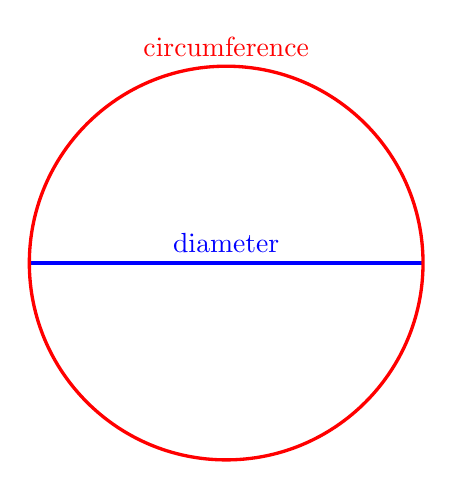
\begin{tikzpicture}[scale=2.5]
\draw[very thick, blue] (-1,0) -- node[above] {diameter} (1,0) coordinate (x axis);
\draw[very thick, red] (0,0) circle (1cm);
\node[red] at (0,1.1) {circumference};
\end{tikzpicture}  
  
  \end{columns}
\end{frame}


\begin{frame}
  \frametitle{What about $\pi = \frac{22}{7}$?}

\pause
\begin{center}
Remember ``Jim'll fix it''?
\pause
\end{center}
\begin{columns}

\column{4 cm}

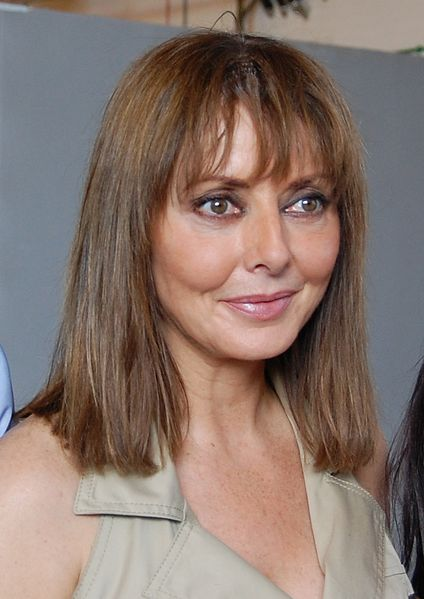
\includegraphics[width = 3 cm]{png/carol_vorderman.jpg}

\small{(Creative Commons \\ commons.wikimedia.org)}

\pause
\column{7 cm}

\[
\frac{22}{7} = 3.142857142857142857\ldots
\]

\pause
What kind of a monster would ask a child to divide 7 into 22 for 50 decimal places, when it is only accurate as $\pi$ for two?
\medskip

\begin{tabular}{cl}
$\frac{22}{7}$ & $3.14285714286\ldots$ \\
$\pi$ & $3.14159265359\ldots$ \\
\end{tabular}

\pause
\medskip
Look closely at the calculation for $\frac{22}{7}$, even with this many decimal places you might notice something.
\end{columns}  
\note{
Sadly, or perhaps otherwise, I couldn't find a YouTube video of this to confirm my memory, but the scarring goes back to 1991.}
\end{frame}


\begin{frame}
  \frametitle{Is everything contained in $\pi$?}

  Once on a while, in Social Media, you will see a nice claim that all possible (finite) sequences of numbers are present in $\pi$ and so it contains your name, everyone's last words, all possible photos of every sunset, and so on and so forth.
  
  \medskip
  \pause
  But is it true?
  
  \medskip
  \pause
  Well, if it is true, it's not because it's irrational
  \[
  0.101001000100001000001\ldots
  \]
  is irrational, and doesn't even contain the number 2, for instance.
\end{frame}


\begin{frame}
  \frametitle{Euler's Number}
  
And $\pi$ isn't the only ubiquitous constant that is irrational. This unusual number is also to be found in many equations.

\[
e = \sum_{n=0}^{\infty} \frac{1}{n!} = 1 + \frac{1}{1} + \frac{1}{1 \times 2} + \frac{1}{1 \times 2 \times 3} + \cdots
\]

The value of $e$ is approximately
\[
e = 2.71828182845904523536028747135266249775724709369995\ldots
\]
\end{frame}

\ifbool{bonus_content}{
\begin{frame}
  \frametitle{The Number of Irrational Numbers}

It's tempting to believe that in some important way there aren't too many of these irrational numbers, that they are hugely outnumbered by the sunlit world of the rationals.

\medskip
\pause
Alas this is not true, not only are there infinitely many of them, but in a precise way there is a bigger infinity of them than the rational numbers.

\medskip
\pause
To put it another way, if all the rationals and irrationals were placed in a bag, then the probability of pulling out a rational would be zero. Nevertheless, we use rationals to approximate our answers in most cases. But the irrational answer is still needed to work out any particular level of accuracy.
\end{frame}
} % bonus_content

\begin{frame}
  \frametitle{The Real Numbers}
  
And so we come to the complete collection of all of that so far, the set of \alert{Real Numbers} ($\mathbb{R}$). Sometimes we just refer to this as the \alert{Real Lines} or the \alert{Continuum}.  
  
\begin{center}
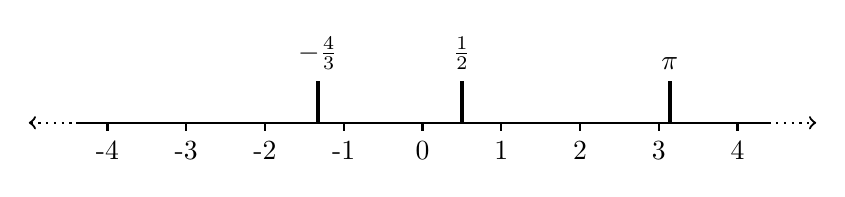
\begin{tikzpicture}[thick]
   \draw[<-, dotted](-5, 0) -- (-4, 0);
   \draw[->, dotted](4, 0) -- (5, 0);
    \draw(-4.4,0)--(4.4,0);
    \foreach \x in {-4, -3, -2, -1, 0, 1, 2, 3, 4}
      \draw(\x,0pt)--(\x,-3pt) node[below] {\x};

    \begin{scope}[ultra thick]
    \draw(0.5,0pt) -- (0.5,15pt) node[above] {$\frac{1}{2}$};
    \draw(3.14,0pt) -- (3.14,15pt) node[above] {$\pi$};
    \draw(-1.33,0pt) -- (-1.33,15pt) node[above] {$-\frac{4}{3}$};
    \end{scope}
\end{tikzpicture}
\end{center}

This has a really pleasing feeling of completeness. Every point on the line is a number, every number is a point on the line. Everything is necessary. And it is sufficient. \pause Yes?
\end{frame}


\begin{frame}
  \frametitle{Square roots continue to deliver pain}
  
What might the square root of 25, $\sqrt{-25}$ be? We are seeking a number, let's call it $z$ so that $z \times z = z^2$ will be $-25$.

\begin{itemize}
\item it cannot be a positive real number, since a positive times a positive is positive (and so cannot possibly be $-25$);
\item it cannot be a negative real number, since similarly a negative times a negative is positive;
\item which leaves zero, but zero times zero is zero, and not $-25$.
\end{itemize}
So, it can't be a Real number. We could give up at this point, but we haven't done that before when we needed negative numbers, or irrational numbers to solve problems.
\end{frame}


\begin{frame}
  \frametitle{Square roots continue to deliver pain}

It turns out we can split this problem up, a bit. We are allowed to split square roots up over multiplication.

\[
\sqrt{-25} = \sqrt{25 \times -1} = \sqrt{25} \times \sqrt{-1} = 5 \times \sqrt{-1}
\]

This has the nice advantage of isolating the tricky bit, this minus sign, in just the $-1$. All square roots of negative numbers can be boiled down in this way. But we have the same problem with $\sqrt{-1}$, it can't be a Real number. What to do?

\[
j = \sqrt{-1}
\]

We make up a new number, $j$ which isn't a Real number that has this value by definition. Now we can say $\sqrt{-25} = 5j$. Does this offend you?
\end{frame}

\begin{frame}
  \frametitle{Where should we put these?}

\begin{center}
\begin{tikzpicture}[thick]
   \draw[<-, dotted](-5, 0) -- (-4, 0);
   \draw[->, dotted](4, 0) -- (5, 0);
    \draw(-4.4,0)--(4.4,0);
    \foreach \x in {-4, -3, -2, -1, 0, 1, 2, 3, 4}
      \draw(\x,0pt)--(\x,-3pt) node[below] {\x};
      
      \pause
      % Let's erase the zero
      \draw[color=white](-0.5,-0.5) rectangle (0.5, -1);
    \foreach \x in { 0}
      \draw(\x,0pt)--(\x,-3pt) node[fill=white, color=white, below] {\x};
      
   \draw[<-, dotted](0, -3) -- (0, -2.4);
   \draw[->, dotted](0, 2.4) -- (0, 3);
    \draw(0,-2.4)--(0,2.4);
    \foreach \x/\y in {-2/-2j, -1/-j, 1/j, 2/2j}
      \draw(-3pt,\x)--(3pt, \x) node[right] {$\y$};
      
    \pause  
    \node at (1,0) {
\includegraphics[width=1cm]{png/cow-clipped.png}};
    \node at (-1,0) {
\includegraphics[width=1cm,angle=180]{png/cow-clipped.png}};

   \pause
    \node at (0,1) {
\includegraphics[width=1cm,angle=90]{png/cow-clipped.png}};
    \node at (0,-1) {
\includegraphics[width=1cm,angle=270]{png/cow-clipped.png}};
\end{tikzpicture}
\end{center}  
\end{frame}


\ifbool{bonus_content}{
\begin{frame}
  \frametitle{More nuisance Square and other Roots}
  
   When we ask what the square root of $1$ is, we find out there are two numbers that square to give one.
  \[
  1 \times 1 = 1 \quad \textrm { and } \quad -1 \times -1 = 1
  \]
  
  When we look for the cube root of 1, i.e. a number which when multiplied by itself three times gives 1, we only get one of these.
  \[
  1 \times 1 \times 1 = 1 \quad \textrm { but } -1 \times -1 \times -1 = -1
  \]
  
This happens due to the way we combine negative signs, as we saw earlier, negative signs ``change direction'' or rather flip the direction, so doing it twice cancels out, three times does not and so on.
\end{frame}
} % bonus_content


\begin{frame}
% Roots of Unity, Real

\begin{tikzpicture}[scale = 1.5,dot/.style={draw,fill,circle,inner sep=2pt}]
  % n = 2
  \begin{scope}
    \draw[thick] (-1.2,0) -- (1.2,0);
	\foreach \x in {-1, 0, 1}
	  \draw(\x,3pt)--(\x,-3pt) node[below] {\x};

	% Draw the roots	
	\node[dot] at (1,0) {};
	\node[dot] at (-1,0) {};
	  
	% Label which root this is
	\node at (-1,1.2) {$\sqrt{1}$ (square root)};
	% A space printed to make space in the diagram to match the next one
	\node at (-1,-1.2) { };
  \end{scope}

  % n = 3
  \begin{scope}[shift={(3,0)}]
    \draw[thick] (-1.2,0) -- (1.2,0);
	\foreach \x in {-1, 0, 1}
	  \draw(\x,3pt)--(\x,-3pt) node[below] {\x};

	% Draw the roots	
	\node[dot] at (1,0) {};
	  
	% Label which root this is
	\node at (-1,1.2) {$\sqrt[3]{1}$ (cube root)};
	% A space printed to make space in the diagram to match the next one
	\node at (-1,-1.2) { };
  \end{scope}

  % n = 4
  \begin{scope}[shift={(0,-3)}]
    \draw[thick] (-1.2,0) -- (1.2,0);
	\foreach \x in {-1, 0, 1}
	  \draw(\x,3pt)--(\x,-3pt) node[below] {\x};

	% Draw the roots	
	\node[dot] at (1,0) {};
	\node[dot] at (-1,0) {};
	  
	% Label which root this is
	\node at (-1,1.2) {$\sqrt[4]{1}$ (fourth root)};
	% A space printed to make space in the diagram to match the next one
	\node at (-1,-1.2) { };
  \end{scope}

  % n = 5
  \begin{scope}[shift={(3,-3)}]
    \draw[thick] (-1.2,0) -- (1.2,0);
	\foreach \x in {-1, 0, 1}
	  \draw(\x,3pt)--(\x,-3pt) node[below] {\x};

	% Draw the roots	
	\node[dot] at (1,0) {};
	  
	% Label which root this is
	\node at (-1,1.2) {$\sqrt[5]{1}$ (fifth root)};
	% A space printed to make space in the diagram to match the next one
	\node at (-1,-1.2) { };
  \end{scope}
\end{tikzpicture}
\end{frame}


\begin{frame}
% Roots of unity, Complex
% Some useful starting points were observed from
% http://tex.stackexchange.com/questions/193402/picture-indicating-the-fifth-roots-of-unity

\begin{tikzpicture}[scale = 1.5,dot/.style={draw,fill,circle,inner sep=2pt}]

  % n = 2
  \begin{scope}
    % Draw axes and labels
    \draw[thick] (-1.2,0) -- (1.2,0);
	\draw[thick] (0,-1.2) -- (0, 1.2);
	\foreach \x in {-1, 1}
	  \draw(\x,3pt)--(\x,-3pt) node[below] {\x};
	\foreach \x/\y in {-1/-j, 1/j}
	  \draw(-3pt,\x)--(3pt,\x) node[right] {$\y$};
	\draw(0,0pt)--(0,-3pt) node[below right] {0};


	% Draw the roots	
	\node[dot] at (1,0) {};
	\foreach \i in {1,...,2} {
    \node[dot,label={\i*360/2-(\i==3)*45:}] (w\i) at (\i*360/2:1) {};
    \draw[very thick, color=ulsterdarkorange,->] (0,0) -- (w\i);
	}
	  
	% Label which root this is
	\node at (-1,1.2) {$\sqrt{1}$ (square root)};
	% A space printed to make space in the diagram to match the next one
	\node at (-1,-1.2) { };
	
	\draw[dotted] (0,0) circle (1cm);
  \end{scope}

  % n = 3
  \begin{scope}[shift={(3,0)}]
    % Draw axes and labels
    \draw[thick] (-1.2,0) -- (1.2,0);
	\draw[thick] (0,-1.2) -- (0, 1.2);
	\foreach \x in {-1, 1}
	  \draw(\x,3pt)--(\x,-3pt) node[below] {\x};
	\foreach \x/\y in {-1/-j, 1/j}
	  \draw(-3pt,\x)--(3pt,\x) node[right] {$\y$};
	\draw(0,0pt)--(0,-3pt) node[below right] {0};

	% Draw the roots	
	\node[dot] at (1,0) {};
	\foreach \i in {1,...,3} {
    \node[dot,label={\i*360/3-(\i==3)*45:}] (w\i) at (\i*360/3:1) {};
    \draw[very thick, color=ulsterdarkorange,->] (0,0) -- (w\i);
  }
	  
	% Label which root this is
	\node at (-1,1.2) {$\sqrt[3]{1}$ (cube root)};
	% A space printed to make space in the diagram to match the next one
	\node at (-1,-1.2) { };
	
	\draw[dotted] (0,0) circle (1cm);
  \end{scope}

  % n = 4
  \begin{scope}[shift={(0,-3)}]
    % Draw axes and labels
    \draw[thick] (-1.2,0) -- (1.2,0);
	\draw[thick] (0,-1.2) -- (0, 1.2);
	\foreach \x in {-1, 1}
	  \draw(\x,3pt)--(\x,-3pt) node[below] {\x};
	\foreach \x/\y in {-1/-j, 1/j}
	  \draw(-3pt,\x)--(3pt,\x) node[right] {$\y$};
	\draw(0,0pt)--(0,-3pt) node[below right] {0};

	% Draw the roots	
	\node[dot] at (1,0) {};
	\node[dot] at (-1,0) {};
	\foreach \i in {1,...,4} {
    \node[dot,label={\i*360/4-(\i==4)*45:}] (w\i) at (\i*360/4:1) {};
    \draw[color=ulsterdarkorange, very thick,->] (0,0) -- (w\i);
  }
	
	  
	% Label which root this is
	\node at (-1,1.2) {$\sqrt[4]{1}$ (fourth root)};
	% A space printed to make space in the diagram to match the next one
	\node at (-1,-1.2) { };
	
	\draw[dotted] (0,0) circle (1cm);
  \end{scope}

  % n = 5
  \begin{scope}[shift={(3,-3)}]
    % Draw axes and labels
    \draw[thick] (-1.2,0) -- (1.2,0);
	\draw[thick] (0,-1.2) -- (0, 1.2);
	\foreach \x in {-1, 1}
	  \draw(\x,3pt)--(\x,-3pt) node[below] {\x};
	\foreach \x/\y in {-1/-j, 1/j}
	  \draw(3pt,\x)--(-3pt,\x) node[left] {$\y$};
	\draw(0,0pt)--(0,-3pt) node[below right] {0};

	% Draw the roots	
	\node[dot] at (1,0) {};
	\foreach \i in {1,...,5} {
    \node[dot,label={\i*360/5-(\i==5)*45:}] (w\i) at (\i*360/5:1) {};
    \draw[very thick, color=ulsterdarkorange,->] (0,0) -- (w\i);
  }
	  
	% Label which root this is
	\node at (-1,1.2) {$\sqrt[5]{1}$ (fifth root)};
	% A space printed to make space in the diagram to match the next one
	\node at (-1,-1.2) { };
	
	\draw[dotted] (0,0) circle (1cm);
  \end{scope}

\end{tikzpicture}
\end{frame}


\begin{frame}
% Roots of unity, complex, but with added cows

\begin{tikzpicture}[scale = 1.5,dot/.style={draw,fill,circle,inner sep=2pt}]

  % n = 2
  \begin{scope}
    % Draw axes and labels
    \draw[thick] (-1.2,0) -- (1.2,0);
	\draw[thick] (0,-1.2) -- (0, 1.2);
	\foreach \x in {-1, 1}
	  \draw(\x,3pt)--(\x,-3pt) node[below] {\x};
	\foreach \x/\y in {-1/-j, 1/j}
	  \draw(-3pt,\x)--(3pt,\x) node[right] {$\y$};
	\draw(0,0pt)--(0,-3pt) node[below right] {0};


	% Draw the roots	
	\node[dot] at (1,0) {};
	\foreach \i in {1,...,2} {
    \node[label={\i*360/2-(\i==3)*45:}, rotate=\i*360/2] (w\i) at (\i*360/2:1) {
\includegraphics[width=1cm]{png/cow-clipped.png}};
    \draw[very thick, color=ulsterdarkorange,->] (0,0) -- (w\i);
	}
	  
	% Label which root this is
	\node at (-1,1.2) {$\sqrt{1}$ (square root)};
	% A space printed to make space in the diagram to match the next one
	\node at (-1,-1.2) { };
	
	\draw[dotted] (0,0) circle (1cm);
  \end{scope}

  % n = 3
  \begin{scope}[shift={(3,0)}]
    % Draw axes and labels
    \draw[thick] (-1.2,0) -- (1.2,0);
	\draw[thick] (0,-1.2) -- (0, 1.2);
	\foreach \x in {-1, 1}
	  \draw(\x,3pt)--(\x,-3pt) node[below] {\x};
	\foreach \x/\y in {-1/-j, 1/j}
	  \draw(-3pt,\x)--(3pt,\x) node[right] {$\y$};
	\draw(0,0pt)--(0,-3pt) node[below right] {0};

	% Draw the roots	
	\node[dot] at (1,0) {};
	\foreach \i in {1,...,3} {
    \node[label={\i*360/3-(\i==3)*45:},rotate=\i*360/3] (w\i) at (\i*360/3:1) {
\includegraphics[width=1cm]{png/cow-clipped.png}};
    \draw[very thick, color=ulsterdarkorange,->] (0,0) -- (w\i);
  }
	  
	% Label which root this is
	\node at (-1,1.2) {$\sqrt[3]{1}$ (cube root)};
	% A space printed to make space in the diagram to match the next one
	\node at (-1,-1.2) { };
	
	\draw[dotted] (0,0) circle (1cm);
  \end{scope}

  % n = 4
  \begin{scope}[shift={(0,-3)}]
    % Draw axes and labels
    \draw[thick] (-1.2,0) -- (1.2,0);
	\draw[thick] (0,-1.2) -- (0, 1.2);
	\foreach \x in {-1, 1}
	  \draw(\x,3pt)--(\x,-3pt) node[below] {\x};
	\foreach \x/\y in {-1/-j, 1/j}
	  \draw(-3pt,\x)--(3pt,\x) node[right] {$\y$};
	\draw(0,0pt)--(0,-3pt) node[below right] {0};

	% Draw the roots	
	\node[dot] at (1,0) {};
	\node[dot] at (-1,0) {};
	\foreach \i in {1,...,4} {
    \node[label={\i*360/4-(\i==4)*45:}, rotate=\i*360/4] (w\i) at (\i*360/4:1) {
\includegraphics[width=1cm]{png/cow-clipped.png}};
    \draw[color=ulsterdarkorange, very thick,->] (0,0) -- (w\i);
  }
	
	  
	% Label which root this is
	\node at (-1,1.2) {$\sqrt[4]{1}$ (fourth root)};
	% A space printed to make space in the diagram to match the next one
	\node at (-1,-1.2) { };
	
	\draw[dotted] (0,0) circle (1cm);
  \end{scope}

  % n = 5
  \begin{scope}[shift={(3,-3)}]
    % Draw axes and labels
    \draw[thick] (-1.2,0) -- (1.2,0);
	\draw[thick] (0,-1.2) -- (0, 1.2);
	\foreach \x in {-1, 1}
	  \draw(\x,3pt)--(\x,-3pt) node[below] {\x};
	\foreach \x/\y in {-1/-j, 1/j}
	  \draw(3pt,\x)--(-3pt,\x) node[left] {$\y$};
	\draw(0,0pt)--(0,-3pt) node[below right] {0};

	% Draw the roots	
	\node[dot] at (1,0) {};
	\foreach \i in {1,...,5} {
    \node[label={\i*360/5-(\i==5)*45:}, rotate=\i*360/5] (w\i) at (\i*360/5:1) {
\includegraphics[width=1cm]{png/cow-clipped.png}};
    \draw[very thick, color=ulsterdarkorange,->] (0,0) -- (w\i);
  }
	  
	% Label which root this is
	\node at (-1,1.2) {$\sqrt[5]{1}$ (fifth root)};
	% A space printed to make space in the diagram to match the next one
	\node at (-1,-1.2) { };
	
	\draw[dotted] (0,0) circle (1cm);
  \end{scope}

\end{tikzpicture}
\end{frame}


\begin{frame}
  \frametitle{Some applications}
  
  \begin{itemize}
    \item Determining the relative size and position of \sout{cows} circuit properties in an AC circuit, using \alert{phasors} (not the ones you set to stun), which also use the ``roots of unity'' in for instance three phase mains electricity.
    \item Solving Differential Equations like this one
    \[
    \frac{d^2x}{dt^2}  + 2\zeta \omega_0 \frac{dx}{dt} + \omega_0^2 x = f(t)
    \]
    \begin{center}
      \begin{tikzpicture}
  \begin{scope}[domain=0:6.7, yscale=1, samples=100]

	\draw[->] (-0.2,0) -- (6.7,0) node[right] {$t$};
	\draw[<->] (0,-1.2) -- (0,1.2) node[above] {$x$};
	\draw[dashed] plot (\x,{e^(-0.3*\x)}) {};
	\draw[dashed] plot (\x,{-e^(-0.3*\x)}) {};
	\draw[color=ulsterdarkorange, thick] plot (\x,{e^(-0.3*\x) *cos(2*\x r)}) {};
	\end{scope}
  \end{tikzpicture}
  \end{center}
  \end{itemize} 
\end{frame}


\section{Circular Functions and Fourier Series}


\begin{frame}
  \frametitle{Origins of Trigonometry}
  
Is this the world's first exam question?  
  
\begin{block}{Rhind Mathematical Papyrus (c. 1680-1620 BC)}
\begin{quote}
"If a pyramid is 250 cubits high and the side of its base 360 cubits long, what is its seked?"
\end{quote}
\end{block}

(For those interested, the \alert{seked} seems to be the cotangent of the angle of the base of the pyramid to its face.)  
\end{frame}


\begin{frame}
  \frametitle{Circular Functions}

\begin{center}
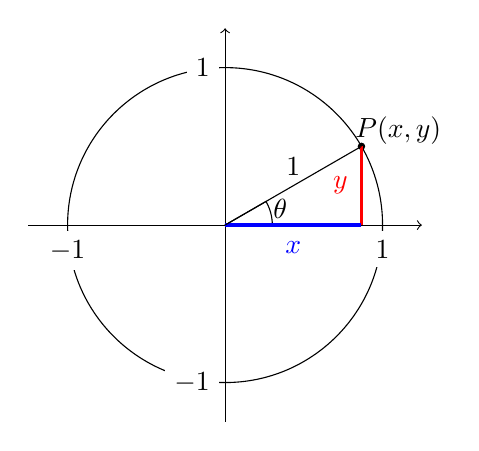
\begin{tikzpicture}[scale=2]

\draw (0,0) -- (3mm,0mm) arc (0:30:3mm) -- cycle;
\node at (0.35,0.1) {$\theta$};

% x, y axis and circle
\draw[->] (-1.25,0) -- (1.25,0) coordinate (x axis);
\draw[->] (0,-1.25) -- (0,1.25) coordinate (y axis);
\draw (0,0) circle (1cm);

% A point P on the circle
\filldraw[fill=black] (0.866cm, 0.5cm) circle (0.02cm);

% Line down from it which is y
\draw[very thick,red]
(30:1cm) -- node[left=1pt,fill=white] {$y$} (30:1cm |- x axis);

% Line across to it which is x
\draw[very thick,blue]
(30:1cm |- x axis) -- node[below=2pt,fill=white] {$x$} (0,0);

% Suppress tan, the unruly cousin
% Line from 1 to intersection of extended line for tan
%\draw[very thick,orange] (1,0) -- node [right=1pt,fill=white]
%{$\displaystyle \tan \theta \color{black}=
%\frac{{\color{red}\sin \theta}}{\color{blue}\cos \theta}$}
%{$t$}
%(intersection of 0,0--30:1cm and 1,0--1,1) coordinate (t);

% Line out to P, which is a radius
\draw (0,0) -- node[above]{$1$} (0.866,0.5);
% Label P itself
\node at (1.1,0.6) {$P (x,y)$};
%\draw (0,0) -- node[above]{$1$}(t);

% Draw -1 and 1 for x and y
\foreach \x/\xtext in {-1,  1}
\draw (\x cm,1pt) -- (\x cm,-1pt) node[anchor=north,fill=white] {$\xtext$};
\foreach \y/\ytext in {-1,  1}
\draw (1pt,\y cm) -- (-1pt,\y cm) node[anchor=east,fill=white] {$\ytext$};
\end{tikzpicture}
\end{center}

($\theta$ is a Greek letter called \alert{theta} that provides the th in many modern words).
\end{frame}


\begin{frame}
  \frametitle{Sine and Cosine}

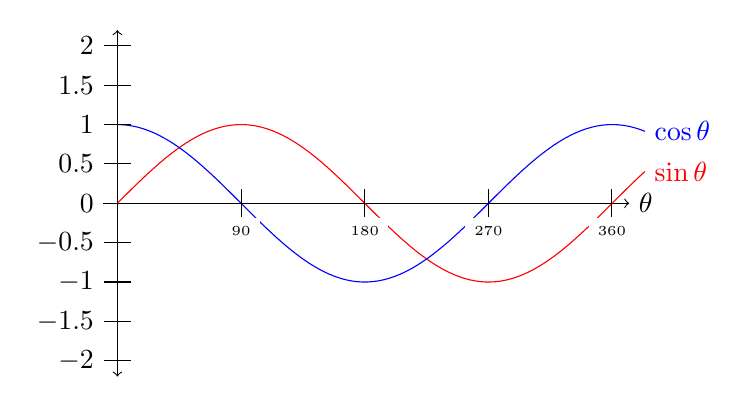
\begin{tikzpicture}[domain=0:6.7, yscale=1, samples=100]

%\draw[very thin,color=gray] (-0.2,-1.1) grid (6.3,3.9);
\draw[->] (-0.2,0) -- (6.5,0) node[right] {$\theta$};
\draw[<->] (0,-2.2) -- (0,2.2);
% sin
\draw[color=red] plot (\x,{sin(\x r)}) node[right] {$\sin \theta$};
% cos
\draw[color=blue] plot (\x,{cos(\x r)}) node[right] {$\cos \theta$};
% ticks on axes
\foreach \x/\xtext in {1.571/90, 3.142/180, 4.712/270, 6.28/360}
\draw (\x cm,5pt) -- (\x cm,-5pt) node[anchor=north, fill=white] {\tiny $\xtext$};
\foreach \y in { -2, -1.5, -1, -0.5, 0, 0.5, 1, 1.5,  2}
\draw (5pt,\y cm) -- (-5pt,\y cm) node[anchor=east, fill=white] { $\y$};
\end{tikzpicture}
\end{frame}


\begin{frame}
  \frametitle{Amplitude and Frequency}

The easiest way to manipulate these is to multiply the whole thing by a number to change the \alert{amplitude} or to multiply the angle by a number to change the \alert{frequency}.

\begin{tikzpicture}
\begin{scope}[domain=0:6.7, yscale=1, samples=500]
%\draw[very thin,color=gray] (-0.2,-1.1) grid (6.3,3.9);
\draw[->] (-0.2,0) -- (6.5,0) node[right] {$\theta$};
\draw[<->] (0,-2.2) -- (0,2.2);
% sin
\draw[color=red] plot (\x,{sin(2*\x r)}) node[right] {$\sin 2\theta$};
% cos
\draw[color=blue] plot (\x,{2*cos(\x r)}) node[right] {$2\cos \theta$};

% ticks on axes
\foreach \x/\xtext in {1.571/90, 3.142/180, 4.712/270, 6.28/360}
\draw (\x cm,5pt) -- (\x cm,-5pt) node[anchor=north, fill=white] {\tiny $\xtext$};
\foreach \y in { -2, -1.5, -1, -0.5, 0, 0.5, 1, 1.5,  2}
\draw (5pt,\y cm) -- (-5pt,\y cm) node[anchor=east, fill=white] { $\y$};

\pause
\draw[color=ulsterdarkorange,thick] plot (\x,{sin(2*\x r) + 2*cos(\x r)}) node[right] {$2\cos \theta + \sin 2\theta$};
\end{scope}
\end{tikzpicture}
\end{frame}


\begin{frame}
  \frametitle{Combining Waves}
  % Saw tooth wave example

\[
\frac{4}{\pi} \left( \sin \theta - \frac{\sin 2 \theta}{2} + \frac{\sin 3 \theta}{3} - \frac{\sin 4 \theta}{4} + \cdots \right)
\]

\begin{tikzpicture}
\begin{scope}[shift={(6,-2)},color=ulsterdarkorange,thick,scale=0.5]
\draw[dotted](6,0) -- (7,1);
\draw(0,0) -- (1,1) -- (1,-1) -- (3,1) -- (3,-1) -- (5, 1) -- (5,-1) -- (6,0);

\draw[dotted,black] (0,1) rectangle (2,-1);
\end{scope}

\begin{scope}[domain=0:6.7, yscale=1, samples=500]
%\draw[very thin,color=gray] (-0.2,-1.1) grid (6.3,3.9);
\draw[->] (-0.2,0) -- (6.5,0) node[right] {$\theta$};
\draw[<->] (0,-2.2) -- (0,2.2);
% sin
%\draw[color=red] plot (\x,{sin(2*\x r)}) node[right] {$\sin 2\theta$};
% cos
%\draw[color=blue] plot (\x,{2*cos(\x r)}) node[right] {$2\cos \theta$};

\draw[color=ulsterdarkorange, thick] (0,0) -- (3.14159, 2) -- (3.14159, -2) -- (6.28,0);

\draw plot (\x, {(4/3.141592) * (sin(\x r) - (1/2)* sin(2*\x r) + (1/3) * sin(3 * \x r) - (1/4) * sin(4 * \x r) + (1/5) * sin(5 * \x r) - (1/6) * sin(6 * \x r) + (1/7) * sin(7 * \x r) -  (1/8) * sin(8 * \x r) + (1/9) * sin(9 * \x r) - (1/10) * sin(10 * \x r))}) node[right] {};
% ticks on axes
\foreach \x/\xtext in {1.571/90, 3.142/180, 4.712/270, 6.28/360}
\draw (\x cm,5pt) -- (\x cm,-5pt) node[anchor=north, fill=white] {\tiny $\xtext$};
\foreach \y in { -2, -1.5, -1, -0.5, 0, 0.5, 1, 1.5,  2}
\draw (5pt,\y cm) -- (-5pt,\y cm) node[anchor=east, fill=white] { $\y$};
\end{scope}\end{tikzpicture}
\end{frame}


\begin{frame}
  \frametitle{Combining Waves}
  % Square wave example

\[
\frac{8}{\pi} \left( \cos \theta - \frac{\cos 3 \theta}{3} + \frac{\cos 5 \theta}{5} - \frac{\cos 7 \theta}{7} + \cdots \right)
\]

\begin{tikzpicture}

\begin{scope}[shift={(6,-2)},color=ulsterdarkorange,thick,scale=0.5]
\draw[dotted](5.5,1) -- (6.5,1);
\draw(0,1) -- (0.5,1) -- (0.5,-1) -- (1.5,-1) -- (1.5,1) -- (2.5, 1) -- (2.5,-1) -- (3.5,-1) -- (3.5,1) -- (4.5,1) -- (4.5, -1) -- (5.5, -1) -- (5.5,1) -- (6,1);

\draw[dotted,black] (0,1) rectangle (2,-1);
\end{scope}

\begin{scope}[domain=0:6.7, yscale=1, samples=500]
%\draw[very thin,color=gray] (-0.2,-1.1) grid (6.3,3.9);
\draw[->] (-0.2,0) -- (6.5,0) node[right] {$\theta$};
\draw[<->] (0,-2.2) -- (0,2.2);
% sin
%\draw[color=red] plot (\x,{sin(2*\x r)}) node[right] {$\sin 2\theta$};
% cos
%\draw[color=blue] plot (\x,{2*cos(\x r)}) node[right] {$2\cos \theta$};

\draw[color=ulsterdarkorange, thick] (0,2) -- (3.14159/2, 2) -- (3.14159/2, -2) -- (3*3.14159/2, -2) -- (3*3.14159/2,2) -- (6.28,2);

\draw plot (\x, {(8/3.141592) * (cos(\x r)  - (1/3) * cos(3 * \x r)  + (1/5) * cos(5 * \x r) - (1/7) * cos(7 * \x r) + (1/9) * cos(9 * \x r))}) node[right] {};
% ticks on axes
\foreach \x/\xtext in {1.571/90, 3.142/180, 4.712/270, 6.28/360}
\draw (\x cm,5pt) -- (\x cm,-5pt) node[anchor=north, fill=white] {\tiny $\xtext$};
\foreach \y in { -2, -1.5, -1, -0.5, 0, 0.5, 1, 1.5,  2}
\draw (5pt,\y cm) -- (-5pt,\y cm) node[anchor=east, fill=white] { $\y$};\end{scope}\end{tikzpicture}
\end{frame}


\begin{frame}
  \frametitle{Frequency and Magnitude}
  % Sawtooth, frequency breakdown

\begin{tikzpicture}
\begin{scope}[yscale=2]
\draw[->] (-0.2,0) -- node[below=1 cm] {frequency} (8.5,0) node[right] {$n$};
\draw[->] (0,-0.2) -- node[left=1.2 cm, rotate=90] {amplitude} (0,2.2);
% ticks on axes
\foreach \x in {1,2,3,4,5,6,7,8}
\draw (\x cm,0pt) -- (\x cm,-5pt) node[anchor=north] {\small $\x$};
\foreach \y in {0, 0.5, 1, 1.5, 2}
\draw (0pt,\y cm) -- (-5pt,\y cm) node[anchor=east, fill=white] { $\y$};

\draw[fill=ulsterdarkorange] (0.9, 0) rectangle (1.1, 1.2732);
\draw[fill=ulsterdarkorange] (1.9, 0) rectangle (2.1, 1.2732/2);
\draw[fill=ulsterdarkorange] (2.9, 0) rectangle (3.1, 1.2732/3);
\draw[fill=ulsterdarkorange] (3.9, 0) rectangle (4.1, 1.2732/4);
\draw[fill=ulsterdarkorange] (4.9, 0) rectangle (5.1, 1.2732/5);
\draw[fill=ulsterdarkorange] (5.9, 0) rectangle (6.1, 1.2732/6);
\draw[fill=ulsterdarkorange] (6.9, 0) rectangle (7.1, 1.2732/7);
\draw[fill=ulsterdarkorange] (7.9, 0) rectangle (8.1, 1.2732/8);
\end{scope}

% Draw the graph reduced and offset to jog memory
\begin{scope}[domain=0:6.7, scale=0.5, samples=500, shift={(10,8)}]
%\draw[very thin,color=gray] (-0.2,-1.1) grid (6.3,3.9);
\draw[->] (-0.2,0) -- (6.5,0) node[right] {$\theta$};
\draw[<->] (0,-2.2) -- (0,2.2);
% sin
%\draw[color=red] plot (\x,{sin(2*\x r)}) node[right] {$\sin 2\theta$};
% cos
%\draw[color=blue] plot (\x,{2*cos(\x r)}) node[right] {$2\cos \theta$};

\draw[color=ulsterdarkorange, thick] (0,0) -- (3.14159, 2) -- (3.14159, -2) -- (6.28,0);

\draw plot (\x, {(4/3.141592) * (sin(\x r) - (1/2)* sin(2*\x r) + (1/3) * sin(3 * \x r) - (1/4) * sin(4 * \x r) + (1/5) * sin(5 * \x r) - (1/6) * sin(6 * \x r) + (1/7) * sin(7 * \x r) -  (1/8) * sin(8 * \x r) + (1/9) * sin(9 * \x r) - (1/10) * sin(10 * \x r))}) node[right] {};
% ticks on axes
\foreach \x/\xtext in {1.571/90, 3.142/180, 4.712/270, 6.28/360}
\draw (\x cm,5pt) -- (\x cm,-5pt) node[anchor=north] {\small $\xtext$};
\foreach \y in { -2, -1, 0, 1, 2}
\draw (5pt,\y cm) -- (-5pt,\y cm) node[anchor=east, fill=white] { $\y$};
\end{scope}
\end{tikzpicture}
\end{frame}


\begin{frame}
  \frametitle{Frequency and Magnitude}
  % Frequency spectrum, square wave

\begin{tikzpicture}
\begin{scope}[yscale=2]
\draw[->] (-0.2,0) -- node[below=1 cm] {frequency} (8.5,0) node[right] {$n$};
\draw[->] (0,-0.2) -- node[left=1.2 cm, rotate=90] {amplitude} (0,2.7);
% ticks on axes
\foreach \x in {1,2,3,4,5,6,7,8}
\draw (\x cm,0pt) -- (\x cm,-5pt) node[anchor=north] {\small $\x$};
\foreach \y in {0, 0.5, 1, 1.5, 2, 2.5}
\draw (0pt,\y cm) -- (-5pt,\y cm) node[anchor=east, fill=white] { $\y$};

\draw[fill=ulsterdarkorange] (0.9, 0) rectangle (1.1, 2.5465);
\draw[fill=ulsterdarkorange] (2.9, 0) rectangle (3.1, 2.5465/3);
\draw[fill=ulsterdarkorange] (4.9, 0) rectangle (5.1, 2.5465/5);
\draw[fill=ulsterdarkorange] (6.9, 0) rectangle (7.1, 2.5465/7);
\end{scope}

% Draw the graph reduced and offset to jog memory
\begin{scope}[domain=0:6.7, scale=0.5, samples=500, shift={(10,8)}]
%\draw[very thin,color=gray] (-0.2,-1.1) grid (6.3,3.9);
\draw[->] (-0.2,0) -- (6.5,0) node[right] {$\theta$};
\draw[<->] (0,-2.2) -- (0,2.2);
% sin
%\draw[color=red] plot (\x,{sin(2*\x r)}) node[right] {$\sin 2\theta$};
% cos
%\draw[color=blue] plot (\x,{2*cos(\x r)}) node[right] {$2\cos \theta$};

\draw[color=ulsterdarkorange, thick] (0,2) -- (3.14159/2, 2) -- (3.14159/2, -2) -- (3*3.14159/2, -2) -- (3*3.14159/2,2) -- (6.28,2);

\draw plot (\x, {(8/3.141592) * (cos(\x r)  - (1/3) * cos(3 * \x r)  + (1/5) * cos(5 * \x r) - (1/7) * cos(7 * \x r) + (1/9) * cos(9 * \x r))}) node[right] {};
% ticks on axes
\foreach \x/\xtext in {1.571/90, 3.142/180, 4.712/270, 6.28/360}
\draw (\x cm,5pt) -- (\x cm,-5pt) node[anchor=north] {\small $\xtext$};
\foreach \y in { -2, -1, 0, 1, 2}
\draw (5pt,\y cm) -- (-5pt,\y cm) node[anchor=east, fill=white] { $\y$};
\end{scope}
\end{tikzpicture}
\end{frame}


\begin{frame}
  \frametitle{Some Applications}
  
  \begin{itemize}
  	\item We can often discard high frequency information and get an acceptable match to the input, allowing us to compress data;
  	\item We can simulate, and interrogate information in many periodic signals, common to life, for instance the ECG;
  	\item This just starts us on the path of using \alert{frequency} rather than \alert{time} as a way to analyse systems. It leads to other techniques such as
  	\begin{itemize}
  	\item The Fourier Transform;
  	\item The Discrete Fourier Transform;
  	\[
  	X_k = \sum_{n=0}^{N-1} x_n \alert{e^{-2 \pi j k n / N}} \quad k \in \mathbb{Z}
  	\]
  	\item The Discrete Cosine Transform (used in compressed photos).
  	\item Laplace transforms, Z-transforms and many others.  	
  	\end{itemize}  
  \end{itemize}
\end{frame}


\section{Implications for Engineering Education}


\begin{frame}
  \frametitle{The Avoidance of Routine}

\begin{block}{A word from a noted educationalist.}
\begin{quote}“A good teacher can never be fixed in a routine... each moment requires a sensitive mind that is constantly changing and constantly adapting. A teacher must never impose this student to fit his favourite pattern \ldots''
%; a good teacher functions as a pointer,\pause exposing his student's vulnerability (and) causing him to explore both internally and finally integrating himself with his being.”
\end{quote}
\end{block}
\pause
\hfill Bruce Lee
\pause

\begin{block}{And another.}
\begin{quote}“You have got to think for yourself. You're all individuals. You're all different.”
\end{quote}
\end{block}
\hfill Brian, Monty Python's Life of Brian

\pause
\begin{columns}
\column{8.5 cm}
\column{1.5 cm}
\begin{block}{}
I'm not
\end{block}
\end{columns}
\end{frame}


\begin{frame}
  \frametitle{Disclaimer: This is not how I lecture...}
  \pause  
  Obvious paradox detected...
  \pause
  \alert{Usually.}
  \pause
  \begin{block}{Student Feedback}
  \begin{quote}
 ``PowerPoint presentations explaining how to do a topic should be banned. I find it very hard to understand if the lecturer is just reading off the board. I prefer Professor Turner's way of teaching, through doing working examples etc. by writing on a page and projecting his page on to the screen. This way of teaching helps me understand better because at least I don't need to worry about the lecturer changing the slide and I'm left with a half written sentence/equation.''
  \end{quote}
  \end{block}
\end{frame}


\begin{frame}
  \frametitle{Stepping Stones}

\begin{block}{Chuck Norris, Bernie Sanders and Donald Trump in a boat}  
Chuck Norris, Bernie Sanders and Donald Trump go out on the lake in a boat. Suddenly, Sanders says, ``I bet I can get to the shore of the lake without getting wet.'' and proceeds to walk over, not getting wet. Chuck Norris decides to give it a try, and also walks across the lake. Trump tries, but immediately falls into the water. ``Do you think we should have told him about the stepping stones'' asks Sanders. Chuck Norris replies, ``What stepping stones?''
\end{block}

\pause
Maths is like this, there are many stones just under the water. Students can be taught to memorise the location of a few tens or hundreds of them. But in reality there is a simple structure which when understood allows a student to walk far without getting wet.  
\end{frame}


\begin{frame}
  \frametitle{Gender, and expectation generally}

\begin{block}{}
\begin{quote}
``What precisely was it you wanted, madam?'' she said.``It’s only that I've left the class doing algebra, and they get restless when they’ve finished.''
\medskip

``Algebra?” said Madam Frout, perforce staring at her own bosom, which no-one else had ever done. ``But that’s far too difficult for seven-year-olds!''
\medskip

``Yes, but I didn’t tell them that and so far they haven’t found out,'' said Susan.\end{quote}
\end{block}
\hfill Terry Pratchett, Thief of Time
\end{frame}


\begin{frame}
  \frametitle{The Hero's Journey}
  
%  \begin{columns}
%  \column{6 cm}
%  \begin{quote}
%  In narratology and comparative mythology, the monomyth, or the \alert{hero's journey}, is the common template of a broad category of tales that involve a hero who goes on an adventure, and in a decisive crisis wins a victory, and then comes home changed or transformed.
%  \end{quote}
%  \hfill From Wikipedia in January 2016
%  
%  \column{6 cm}
  \begin{center}
  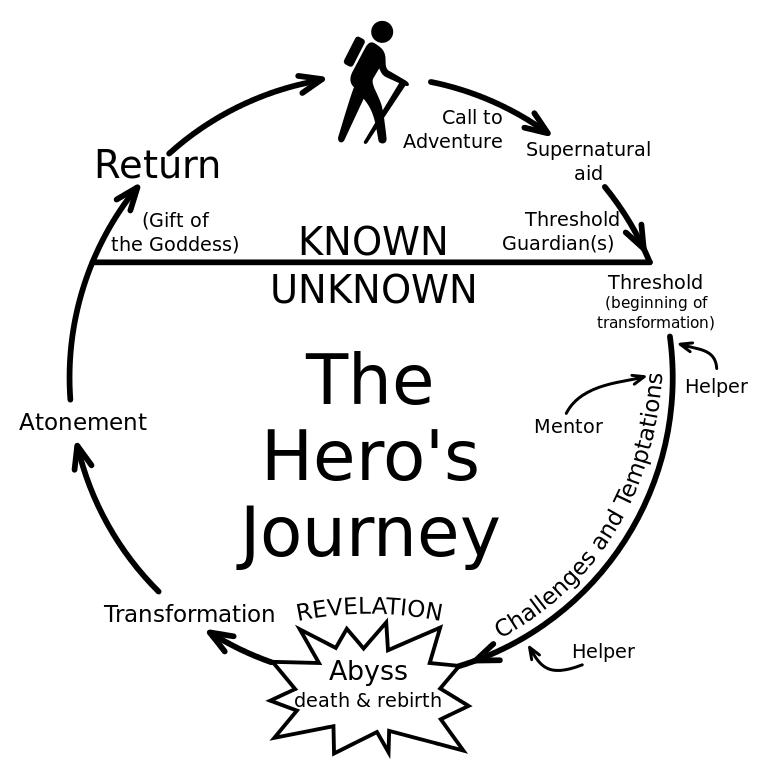
\includegraphics[width= 6 cm]{png/Heroesjourney.png}
  
  \small{(Creative Commons \\ commons.wikimedia.org)}

  \end{center}
%  \end{columns}
\end{frame}


\begin{frame}
\begin{center}
\begin{block}{}
\begin{quote}
``We live on an island surrounded by a sea of ignorance. As our island of knowledge grows, so does the shore of our ignorance.''
\end{quote}
\end{block}
\hfill John Archibald Wheeler
\end{center}

\pause
\bigskip
Reminder, extra content at \url{http://www.piglets.org/inaugural}

\end{frame}
\end{document}

% No, really...